\chapter{Fejlesztői dokumentáció}
\label{ch:impl}
 A következő fejezetben az alkalmazást fejlesztői szemszögből mutatom be. Részletesen kitérek az alkalmazás felépítésére, a használt technológiákra, az adatbázis-struktúrára, valamint a fejlesztés során követett elvekre és megoldásokra.

\section{Architektúra}
\begin{itemize}
	\item Frontend: HTML\footnote{Mivel a C\# projekten
		belül lett létrehozva a frontend is, ezért a .html helyett .cshtml
		kiterjesztésű fájlok vannak. Ezek annyiban különböznek a 
		HTML-től, hogy vannak bizonyos tagek, kulcsszavak, melyekkel
		különleges dolgokat tudunk csinálni. A Frontend című fejezetben kerül ez a téma bővebb kifejtésre.}/CSS/JavaScript (és Bootstrap)
	\item Backend: C\# (ASP.NET Web App (Razor Pages))
	\item Adatbázis: MySQL relációs adatbázis
\end{itemize}

\begin{figure}[H]
	\centering
	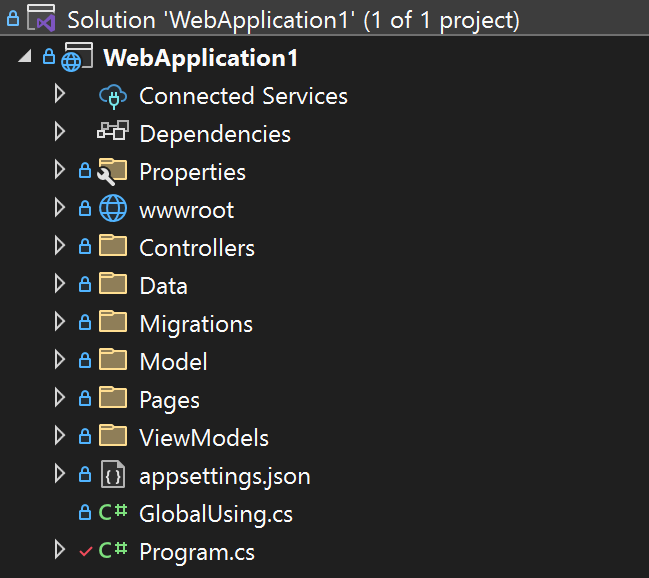
\includegraphics[height=220px]{img/solution-explorer-screenshot}
	\caption{Projekt struktúra}
	\label{fig:project-structure}
\end{figure}

\subsection{Architektúra leírása}
Ahogy a \ref{fig:project-structure}. ábrán is látható, az egész webalkalmazás egy projekten belül lett kialakítva. A .NET-es integrált frontend és backend fejlesztés hatalmas előnye a rendszerezettség, a szabályszerű kommunikáció az egyes rétegek között (illetve ezen rétegek helyes elkülönölése), és a rengeteg beépített segédfüggvény/konfiguráció/cshtml tag. Kiemelném még a modellek használatát is, amelyek egyszerűbb és biztonságosabb (például SQL injection elleni védelem) adatbázis kezelést biztosítanak.

Az egyes route-ok konfigurálása is meglehetősen letisztult ebben a keretrendszerben. A "Pages" mappa\footnote{A "Pages" mappa, ahogy a neve is mutatja, tartalmazza a weboldal egyes oldalait. Bővebb kifejtés a Frontend című fejezetben.} fájlstruktúrája alapján automatikusan létrejönnek a route-ok, ha a "Program.cs"-ben megadjuk a programnak, hogy hozza létre őket:

\lstset{caption={Route-ok konfigurálása}, label=src:routing}
\begin{lstlisting}[language={[Sharp]C}]
	app.UseRouting();
\end{lstlisting}

A frontend és a backend közötti hagyományos JavaScript segítségével történő kommunikáción kívül, a cshtml formátum miatt lehetőség nyílik egyszerűbb esetekre közvetlen kapcsolatot is létesíteni a backend és a frontend között. Például:

\lstset{caption={Frontend modell egy alkalmazása}, label=src:model}
\begin{lstlisting}[language={HTML}]
	<h1>Username</h1>
	<p>@Model.UserData.Username</p>
\end{lstlisting}

Itt ugye mint látható a modellből tudunk adatot lekérdezni.
De mi is a "Model" pontosan? Ugyebár az ASP .NET Web App keretrendszer úgy működik, hogy minden oldal (Razor page) egy .cshtml és egy .cs fájl együtteséből áll össze. A .cs kiterjesztésű fájl az adott oldal modellje. Itt definiálhatunk adatszerkezeteket és függvényeket, mint például az OnGet() és OnPost(), amelyek beépített (opcionális) metódusok, és ahogy a nevük is mutatja,
az oldalról érkező GET és POST requesteket kezelik. Tehát például,
ha az adott oldalon egy darab form-unk van, amit POST metódussal
be akarunk küldeni a szervernek, ezt JS (JavaScript) kód írása nélkül biztonságosan meg tudjuk tenni.

\section{Backend}

A következő fejezetben az alkalmazás backend architektúráját mutatom be, kifejtve az egyes elemek funkcióit és használatát.

\subsection{appsettings.json}

Az appsettings.json egy konfigurációs
fájl. Ebben lehet alkalmazásszintű beállításokat tárolni, például:
adatbáziskapcsolati stringeket,
API kulcsokat,
logolási beállításokat,
vagy bármilyen egyedi, fejlesztő által definiált értéket.
Az értékeket a program bármely részén könnyen ki lehet olvasni (szótár szintaktika használatával)  (pl. Configuration["Kulcs"]). Ez segít elkülöníteni a kódot a
konfigurációtól, így könnyebb a karbantartás, és egyszerűen kezelhető a környezetenkénti
eltérés (pl. fejlesztői vs. éles környezet).

\subsection{Program.cs}
Ez a fő program fájl, és egyben az alkalmazás belépési pontja. Ebben készítjük
elő a webalkalmazásunk tulajdonságait (persze a Razor Pages egyszerűségének
hála ez nem sok plusz feladattal jár, csupán a helyes függvényeket
kell meghívni helyes sorrendben, attól függően, hogy hogyan
akarjuk konfigurálni az alkalmazást). Itt lehet beállítani a
korábban említett routing-ot, az autentikációt, a cookie-kat,
a session-t, a fejlesztői és éles környezeteket, és még sok minden mást. Itt tudjuk felkonfigurálni a modellt, az adatbázist
és az oldalakat (Pages) is. ezután az app.Run() függvény hívással
tudjuk ténylegesen elindítani a weboldalt.

\subsection{Modellek}
Minden adatbázis táblának létrehozunk egy modellt
(bővebb kifejtés az "adatbázis" pontban). Ezek mind C\# osztályok
táblánként, és minden oszlop egy külön propertynek feleltethető meg.

\subsection{API}
Az ASP.NET-es struktúra úgy működik, hogy miután a 
Program.cs-ben felkonfiguráltuk a szükséges dolgokat, megalkottuk a modelleket, létrehoztuk a HTML lapokat, már csak
egy fontos dolog maradt hátra. A frontend-backend kommunikáció.
Említés esett már arról, hogy egyszerűbb esetekben ezt a HTML-ben
bizonyos tagekkel meg tudjuk tenni, de a nem triviális esetek
megoldására is egyszerű módot kinál a .NET. A Controllers
mappában minden modellnek (vagyis minden adatbázis táblának)
létrehozunk egy Controller fájlt is. Ebben fogunk API-végpontokat
definiálni, melyeket a frontenden JavaScript segítségével tudunk
meghívni, és ezáltal adatot közvetíteni a felhasználó és a szerver
között (oda-vissza). Az API-endpointok tesztelésére és leírására
egy hasznos, szintén beépített, megoldást használhatunk, a Swaggert.
Ezt is a Program.cs fájlban állíthatjuk be.\footnote{Szigorúan csak 
Development módban jelenjen meg, adatvédelmi/adat hitelességi okokból.} A Swagger az alkalmazás API-végpontjainak dokumentációja, amely lehetőséget biztosít az egyes végpontok közvetlen tesztelésére is.
\section{Frontend}
Térjünk át a frontend réteg alkotóelemeire, és ezek működésére. Itt is komponensenként fogom bemutatni a felhasznált technológiákat.

\subsection{Layout}
A "Pages" mappa tartalmazza az oldalakat. A keretrendszer ugyebár úgy működik, hogy minden oldal (Razor page) egy .cshtml és egy .cs
fájl együtteséből áll össze. A Pages mappa ezeket a párosokat tartalmazza, további kisebb mappákra bontva a funkció csoportok alapján. Az alább mellékelt ábrából (\ref{fig:pages-structure}. ábra) látható tehát, hogy például a bejelentkező felületet a következő linken tudjuk elérni: "localhost:<<port>>/Account/Login".

\begin{figure}[H]
	\centering
	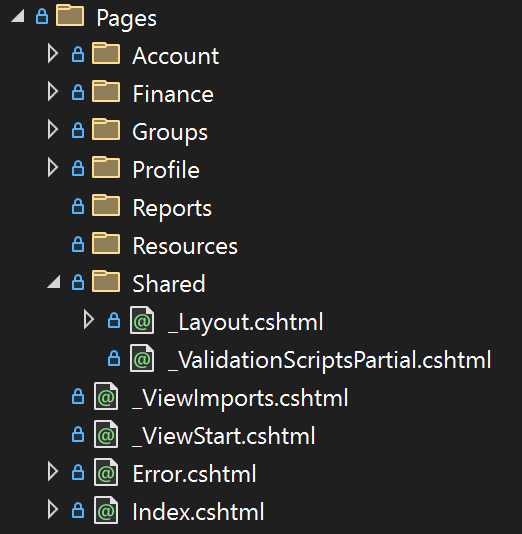
\includegraphics[height=240px]{img/solution-explorer-pages-screenshot}
	\caption{Pages struktúra}
	\label{fig:pages-structure}
\end{figure}

Találhatók még ebben a mappában egyéb segédfájlok is, mint például az Error.cshtml, ami az esetleges hibák esetén jelenik meg. Kiemelendő még a Shared mappa, amiben található egy Layout.cshtml fájl is (modell nélkül). Ez, ahogy a neve is mutatja egy alap sablont biztosít az alkalmazás felületének. A weboldal egy (a képernyő baloldán lévő) főmenüből, egy kis (az oldal tetején található) menüsávból, a fő tartalmi részből áll, illetve egy footer részből áll. A footer és a menüsávok kódját tartalmazza a Layout.cshtml között a tartalomnak "kihagyott" rész: 
\lstset{caption={Layout extension ASP.NET keretrendszerben}, label=src:csharp}
\begin{lstlisting}[language={HTML}]
	<div class="container-fluid">
	@RenderBody()
	</div>
\end{lstlisting}

A RenderBody() függvény (szintén beépített .NET metódus)
behelyezi az adott oldal HTML kódját ebbe a div HTML elembe. Ez
automatikusan megtörténik az összes oldal esetében amelyre
navigál a felhasználó. Ha valami miatt éppen nem ezt a sablont akarjuk követni egy oldalunkkal (például: Bejelentkező felület), akkor az adott oldal HTML kódjába beírhatjuk hogy ne sablont kövessen:

\begin{lstlisting}[language={[Sharp]C}]
	@{
		Layout = null; // Remove layout if you want a standalone page
	}
\end{lstlisting}

\subsection{static}
A "wwwroot" mappában található az összes statikus erőforrás (static resource). Itt a hagyományosan használt mappastruktúrát követtem az alkalmazás készítésekor, azaz létre lettek hozva a következő mappák:
\begin{itemize}
	\item "js": JavaScript kódok
	\item "css": CSS stylesheetek
	\item "img": Képek  
\end{itemize}
A frontend rész formázását Bootstrap keretrendszer felhasználásával valósítottam meg. Ezt úgy importáltam a projektbe, hogy a kész CSS/JS fileok vannak letöltve ugyanide, a wwwroot mappába, ezen kívül egy külső hivatkozás van egy betűtípusra. 

\section{Adatbázis}
Az alkalmazás működésének egyik alapvető pillére az adatbázis, amely a rendszerben tárolt információk strukturált kezelését, hosszú távú perzisztenciáját és elérhetőségét biztosítja. Az adatbázis szerkezete úgy került kialakításra, hogy az hatékonyan támogassa az alkalmazás funkcionális igényeit, miközben jól skálázható és könnyen karbantartható maradjon.

Az adatbázis relációs modellre épül, és az adatok külön táblákban kerülnek tárolásra, melyeket kulcsok és kapcsolat típusok kötnek össze.

\subsection{Szerkezet}
Az alkalmazás adatbázisa egy localhoston futó MySQL adatbázis.
A MySQL-t sok szempont miatt szokták kisebb alkalmazásokhoz
használni, ezek közé tartozik például az a nem elhanyagolható
indok, hogy teljesen ingyenes a használata. Illetve szintén
az egyszerűségét tudnám kiemelni, és a kompatibilitását az ASP.NET keretrendszerrel. Egy darab adatbázis lett létrehozva, azon belül több tábla található, melyek természetesen kapcsolódnak egymáshoz. Az adatmodell a relációs adatbázisok normalizálási elvein alapul, és a harmadik normálformáig (3NF) került kialakításra.
A szerkezetet és a logikai kapcsolatokat az egyes táblák között a \ref{fig:database-structure}. ábra szemlélteti. A táblák részletes leírását pedig a \ref{tab:db-desc}. táblázat tartalmazza.

\begin{figure}[H]
	\centering
	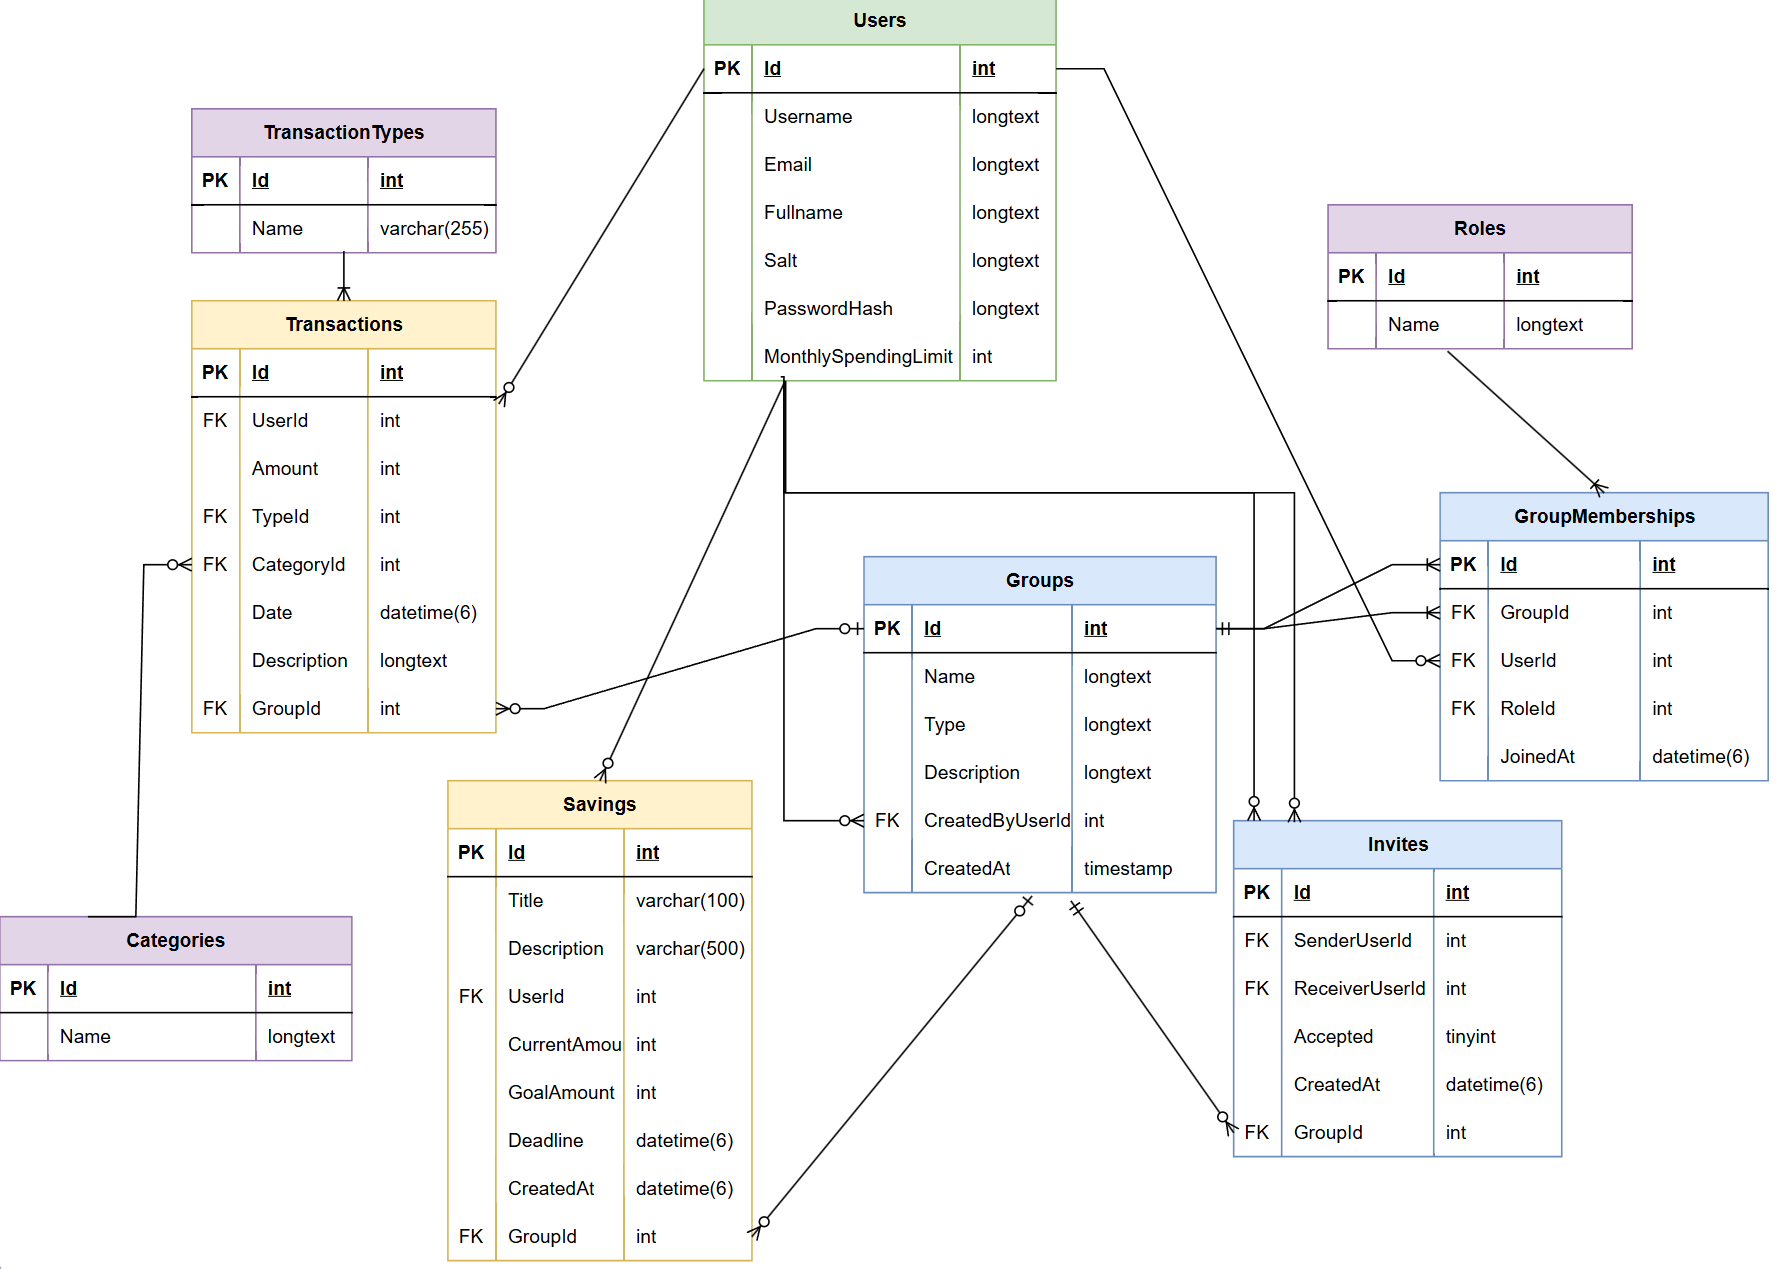
\includegraphics[height=320px]{img/0000}
	\caption{Adatbázis struktúra}
	\label{fig:database-structure}
\end{figure}

\begin{longtable}{ | m{0.25\textwidth} | m{0.65\textwidth} | }
	\hline
	\textbf{Tábla} & \textbf{Leírás} \\
	\hline
	\endfirsthead
	
	\hline
	\textbf{Tábla} & \textbf{Leírás} \\
	\hline
	\endhead
	
	\hline
	\endfoot
	
	\hline
	\caption{Adatbázis táblák magyarázata} \label{tab:db-desc} \\
	\endlastfoot
	
	Users & A rendszer felhasználóit tartalmazza. Itt tároljuk az alapvető adatokat (felhasználónév, e-mail, teljes név), a hitelesítéshez szükséges információkat (salt és jelszóhash), valamint a havi költési limitet is. \\
	\hline
	Groups & A csoportokat kezeli, amelyekbe a felhasználók beléphetnek. Minden csoportnak van neve, típusa (pl. család, baráti társaság, ez szabad szöveges érték), leírása, létrehozó felhasználója és létrehozási dátuma. \\
	\hline
	GroupMemberships & A felhasználók csoporttagságait rögzíti. Megmutatja, hogy ki melyik csoporthoz tartozik, milyen szerepkörben (pl. admin vagy tag), és mióta tagja a csoportnak. \\
	\hline
	Roles & Az egyes csoporttagságokhoz rendelhető szerepköröket definiálja, például adminisztrátor vagy sima tag. A szerepkörök szabályozzák a felhasználók jogosultságait a csoportban. A csoport létrehozójának "Admin" jogköre lesz automatikusan, a felvett tagnak pedig "Member".\\
	\hline
	Transactions & A felhasználók által rögzített pénzügyi tranzakciókat tárolja. Minden tranzakcióhoz tartozik összeg, típus (bevétel vagy kiadás), kategória (pl. étel, szórakozás), dátum, leírás, és adott esetben kapcsolódó csoport is. A "GroupId" értéke null, ha személyes a tranzakció. \\
	\hline
	TransactionTypes & A tranzakciók típusait (bevétel, kiadás) határozza meg. \\
	\hline
	Categories & A tranzakciókhoz tartozó kategóriákat tartalmazza, mint például élelmiszer, közlekedés, szórakozás stb. Segíti a kiadások és bevételek részletesebb elemzését. \\
	\hline
	Savings & A felhasználók által kitűzött megtakarítási célokat tárolja. A célösszeg és a határidő opcionális adatok, tehát lehet null értékük. A "GroupId" értéke is null, ha személyes megtakarítás. \\
	\hline
	Invites & A csoportokba történő meghívásokat kezeli. Menti, hogy ki küldött meghívót kinek, melyik csoportba, és hogy a meghívás elfogadásra került-e. Az elfogadott meghívók "Accepted" értéke 1-re vált a default 0-ról. Elutasítás esetén a meghívó törlődik a táblából. \\
\end{longtable}



\subsection{Backend - Adatbázis kapcsolat}
A backend és az adatbázis kapcsolata relatív egyszerűen megvalósítható az ASP.NET keretrendszerben.
A NuGet package managerből az EntityFramework egyes csomagjait,
illetve a MySQL Connector csomagot letöltve már alig van
dolgunk. Az appsettings.json fájlban tudjuk a connection
stringet definiálni.

\lstset{caption={Adatbázis Connection String}, label=src:connstring}
\begin{lstlisting}[language={HTML}]
	"ConnectionStrings": {
		"MySqlConnection": "server=localhost;port=3306;database=betterspend;user=root;password=<<password>>;"
	}
\end{lstlisting}

majd a Program.cs fájlban tudunk ténylegesen csatlakozni:

\lstset{caption={Program.cs: Adatbázis csatlakozás}, label=src:csharp}
\begin{lstlisting}[language={[Sharp]C}]
	// Get MySQL connection string from configuration
	string connectionString = builder.Configuration.GetConnectionString("MySqlConnection");
	
	// Add DB Context to the application
	builder.Services.AddDbContext<ApplicationDbContext>(options =>
	{
		options.UseMySql(connectionString, ServerVersion.AutoDetect(connectionString));
	});
\end{lstlisting}

A tényleges adatbázis modellje:

\lstset{caption={Adatbázis modell}, label=src:dbmodel}
\begin{lstlisting}[language={[Sharp]C}]
	using WebApplication1.Model;
	namespace WebApplication1.Data
	{
		public class ApplicationDbContext : DbContext
		{
			public ApplicationDbContext(DbContextOptions<ApplicationDbContext> options)
			: base(options)
			{
			}
			
			public DbSet<User> Users { get; set; }
			public DbSet<Transaction> Transactions { get; set; }
			public DbSet<Category> Categories { get; set; }
			
		}
	}
\end{lstlisting}

Ezután már az adatbázisunk össze van kötve teljesen az alkalmazással. ASP.NET-ben közvetlenül az adatbázishoz (lekérdezésekkel, parancsokkal) nem tudunk hozzáférni. Amihez hozzá tudunk férni azok a modell fájlok (pl. Model/User). Ezeket tudjuk módosítani LINQ segítségével egyszerűen, és ez szinkronizálni fogja
a tényleges adatbázisunkkal.

\subsection{Migrations}
A későbbi fejlesztések során migrációkat használhatunk az adatbázis verziókövetésére és a változtatások biztonságos, konzisztens bevezetésére. A migrációk használata Entity Framework Core segítségével történik, ahol a DbContext osztály definiálja az adatbázis szerkezetét. A módosításokat a dotnet ef migrations add paranccsal lehet rögzíteni, majd a dotnet ef database update parancs segítségével alkalmazni az adatbázisra. Ez lehetővé teszi a séma változásainak verziókövetését és biztonságos frissítését.

\section{Tesztek}
\begin{table}[h!]
	\centering
	\begin{tabular}{|l|p{10cm}|}
		\hline
		\textbf{Teszteset azonosító} & TC001 \\ \hline
		\textbf{Funkció} & Regisztráció \\ \hline
		\textbf{Bemenet} & Valid e-mail cím, egyedi felhasználónév, teljes név, jelszó \\ \hline
		\textbf{Elvárt eredmény} & Sikeres regisztráció, átirányítás a bejelentkezés felületre, visszajelző üzenet a felhasználónak \\ \hline
		\textbf{Tényleges eredmény} & Megfelel az elvárt eredménynek\\ \hline
	\end{tabular}
	\caption{Sikeres regisztráció}
	\label{tab:manual_testcase_registration}
\end{table}
\begin{table}[h!]
	\centering
	\begin{tabular}{|l|p{10cm}|}
		\hline
		\textbf{Teszteset azonosító} & TC002 \\ \hline
		\textbf{Funkció} & Regisztráció \\ \hline
		\textbf{Bemenet} & Üres mezők beküldése vagy invalid e-mail cím, vagy nem elég erős jelszó \\ \hline
		\textbf{Elvárt eredmény} & Hibajelzés, regisztráció sikertelen \\ \hline
		\textbf{Tényleges eredmény} & Megfelel az elvárt eredménynek \\ \hline
	\end{tabular}
	\caption{Sikertelen regisztráció}
	\label{tab:regisztracio_ures}
\end{table}

\begin{table}[h!]
	\centering
	\begin{tabular}{|l|p{10cm}|}
		\hline
		\textbf{Teszteset azonosító} & TC003 \\ \hline
		\textbf{Funkció} & Bejelentkezés \\ \hline
		\textbf{Bemenet} & Helyes felhasználónév - jelszó páros megadása \\ \hline
		\textbf{Elvárt eredmény} & Belépteti a felhasználót az oldalra \\ \hline
		\textbf{Tényleges eredmény} & Megfelel az elvárt eredménynek \\ \hline
	\end{tabular}
	\caption{Sikeres bejelentkezés}
	\label{tab:bejelentkezes_hibas_adatokkal}
\end{table}

\begin{table}[h!]
	\centering
	\begin{tabular}{|l|p{10cm}|}
		\hline
		\textbf{Teszteset azonosító} & TC004 \\ \hline
		\textbf{Funkció} & Bejelentkezés \\ \hline
		\textbf{Bemenet} & Üres mezők beküldése, vagy helytelen felhasználónév-jelszó páros \\ \hline
		\textbf{Elvárt eredmény} & Hibajelzés, a bejelentkezés sikertelen\\ \hline
		\textbf{Tényleges eredmény} & Megfelel az elvárt eredménynek \\ \hline
	\end{tabular}
	\caption{Sikertelen bejelentkezés}
	\label{tab:bejelentkezes_ures}
\end{table}

\begin{table}[h!]
	\centering
	\begin{tabular}{|l|p{10cm}|}
		\hline
		\textbf{Teszteset azonosító} & TC005 \\ \hline
		\textbf{Funkció} & Profil oldal - adatok módosítása \\ \hline
		\textbf{Bemenet} & Új, egyedi felhasználónév megadása VAGY új, valid e-mail cím megadása VAGY új teljes név megadása \\ \hline
		\textbf{Elvárt eredmény} & Sikeres módosítás \\ \hline
		\textbf{Tényleges eredmény} & Megfelel az elvárt eredménynek \\ \hline
	\end{tabular}
	\caption{Személyes adatok sikeres módosítása}
	\label{tab:profil_felhasznalonev_modositas}
\end{table}

\begin{table}[h!]
	\centering
	\begin{tabular}{|l|p{10cm}|}
		\hline
		\textbf{Teszteset azonosító} & TC006 \\ \hline
		\textbf{Funkció} & Profil oldal - adatok módosítása \\ \hline
		\textbf{Bemenet} & Helytelen e-mail cím megadás, foglalt felhasználónév megadás, üres mező beküldése \\ \hline
		\textbf{Elvárt eredmény} & Hibajelzés, a módosítás nem lép érvénybe \\ \hline
		\textbf{Tényleges eredmény} & Megfelel az elvárt eredménynek \\ \hline
	\end{tabular}
	\caption{Személyes adatok sikertelen módosítása}
	\label{tab:profil_felhasznalonev_foglalt}
\end{table}


\begin{table}[h!]
	\centering
	\begin{tabular}{|l|p{10cm}|}
		\hline
		\textbf{Teszteset azonosító} & TC007 \\ \hline
		\textbf{Funkció} & Profil oldal - Jelszó módosítása \\ \hline
		\textbf{Bemenet} & Helyes régi jelszó, új jelszó, új jelszó megerősítése egyezően, új jelsző elég erős \\ \hline
		\textbf{Elvárt eredmény} & Sikeres jelszóváltás, visszajelzés a felhasználónak \\ \hline
		\textbf{Tényleges eredmény} & Megfelel az elvárt eredménynek \\ \hline
	\end{tabular}
	\caption{Sikeres jelszó modósítás}
	\label{tab:profil_jelszo_modositas}
\end{table}

\begin{table}[h!]
	\centering
	\begin{tabular}{|l|p{10cm}|}
		\hline
		\textbf{Teszteset azonosító} & TC008 \\ \hline
		\textbf{Funkció} & Profil oldal - Jelszó módosítása \\ \hline
		\textbf{Bemenet} & Helytelen régi jelszó, új jelszó és megerősítés nem egyező, nem elég erős új jelszó \\ \hline
		\textbf{Elvárt eredmény} & Hibajelzés, módosítás nem lép érvénybe \\ \hline
		\textbf{Tényleges eredmény} & Megfelel az elvárt eredménynek \\ \hline
	\end{tabular}
	\caption{Sikertelen jelszó módosítás}
	\label{tab:jelszo_modositas_rossz_regi}
\end{table}

\begin{table}[h!]
	\centering
	\begin{tabular}{|l|p{10cm}|}
		\hline
		\textbf{Teszteset azonosító} & TC009 \\ \hline
		\textbf{Funkció} & Új bevétel rögzítése \\ \hline
		\textbf{Bemenet} & Helyes amount (pl. 5000) és description (pl. "Fizetés") \\ \hline
		\textbf{Elvárt eredmény} & Sikeres mentés, üzenet: "Transaction saved!" \\ \hline
		\textbf{Tényleges eredmény} & Megfelel az elvárt eredménynek \\ \hline
	\end{tabular}
	\caption{Új bevétel helyes adatokkal}
	\label{tab:uj_bevetel_helyes}
\end{table}

\begin{table}[h!]
	\centering
	\begin{tabular}{|l|p{10cm}|}
		\hline
		\textbf{Teszteset azonosító} & TC010 \\ \hline
		\textbf{Funkció} & Új bevétel rögzítése \\ \hline
		\textbf{Bemenet} & Üres vagy hibás amount/description mezők \\ \hline
		\textbf{Elvárt eredmény} & Hibajelzés: "Failed to create transaction!" (Tranzakció mentése sikertelen.) \\ \hline
		\textbf{Tényleges eredmény} & Megfelel az elvárt eredménynek \\ \hline
	\end{tabular}
	\caption{Új bevétel hibás adatokkal}
	\label{tab:uj_bevetel_hibas}
\end{table}

\begin{table}[h!]
	\centering
	\begin{tabular}{|l|p{10cm}|}
		\hline
		\textbf{Teszteset azonosító} & TC011 \\ \hline
		\textbf{Funkció} & Kiadás rögzítése, ha havi limit = 0 \\ \hline
		\textbf{Bemenet} & Új kiadás mentése 0 költési limit mellett \\ \hline
		\textbf{Elvárt eredmény} & Üzenet: "Transaction saved!" (limit státusz nélkül) \\ \hline
		\textbf{Tényleges eredmény} & Megfelel az elvárt eredménynek \\ \hline
	\end{tabular}
	\caption{Kiadás rögzítése havi limit nélkül}
	\label{tab:kiadas_limit_nelkul}
\end{table}

\begin{table}[h!]
	\centering
	\begin{tabular}{|l|p{10cm}|}
		\hline
		\textbf{Teszteset azonosító} & TC012 \\ \hline
		\textbf{Funkció} & Kiadás rögzítése, ha van havi limit \\ \hline
		\textbf{Bemenet} & Új kiadás mentése havi limit mellett \\ \hline
		\textbf{Elvárt eredmény} & Limit státusz megjelenik: zöld (ha van keret), sárga (ha túllépés történt) \\ \hline
		\textbf{Tényleges eredmény} & Megfelel az elvárt eredménynek \\ \hline
	\end{tabular}
	\caption{Kiadás rögzítése havi limittel}
	\label{tab:kiadas_limit_ellenorzes}
\end{table}

\begin{table}[h!]
	\centering
	\begin{tabular}{|l|p{10cm}|}
		\hline
		\textbf{Teszteset azonosító} & TC013 \\ \hline
		\textbf{Funkció} & Előzmény táblázat ellenőrzése \\ \hline
		\textbf{Bemenet} & Új bevétel/kiadás rögzítése \\ \hline
		\textbf{Elvárt eredmény} & Az új tranzakció megjelenik az előzmények között \\ \hline
		\textbf{Tényleges eredmény} & Megfelel az elvárt eredménynek \\ \hline
	\end{tabular}
	\caption{Új tranzakció megjelenése az előzmények között}
	\label{tab:elozmeny_tabla}
\end{table}

\begin{table}[h!]
	\centering
	\begin{tabular}{|l|p{10cm}|}
		\hline
		\textbf{Teszteset azonosító} & TC014 \\ \hline
		\textbf{Funkció} & CSV batch feltöltés \\ \hline
		\textbf{Bemenet} & Helyes formátumú CSV fájl feltöltése (típus, kategória, leírás, összeg, dátum) \\ \hline
		\textbf{Elvárt eredmény} & Minden sor külön tranzakcióként mentésre kerül, üzenet: "Transactions saved!" (Tranzakciók elmentve!) \\ \hline
		\textbf{Tényleges eredmény} & Megfelel az elvárt eredménynek \\ \hline
	\end{tabular}
	\caption{CSV batch feltöltés helyes fájllal}
	\label{tab:csv_feltoltes}
\end{table}

\begin{table}[h!]
	\centering
	\begin{tabular}{|l|p{10cm}|}
		\hline
		\textbf{Teszteset azonosító} & TC015 \\ \hline
		\textbf{Funkció} & CSV batch feltöltés \\ \hline
		\textbf{Bemenet} & Helytelen formátumú CSV fájl feltöltése (típus, kategória, leírás, összeg, dátum) \\ \hline
		\textbf{Elvárt eredmény} & Hibaüzenet: "Error! <<a pontos hiba>>" (Hiba!) \\ \hline
		\textbf{Tényleges eredmény} & Megfelel az elvárt eredménynek \\ \hline
	\end{tabular}
	\caption{CSV batch feltöltés helytelen fájllal}
	\label{tab:csv_feltoltes_helytelen}
\end{table}

\begin{table}[h!]
	\centering
	\begin{tabular}{|l|p{10cm}|}
		\hline
		\textbf{Teszteset azonosító} & TC016 \\ \hline
		\textbf{Funkció} & Havi költési limit módosítása \\ \hline
		\textbf{Bemenet} & Új poitív egész költési limit megadása (pl. 100000) \\ \hline
		\textbf{Elvárt eredmény} & Sikeres módosítás, limit frissítése az adatbázisban \\ \hline
		\textbf{Tényleges eredmény} & Megfelel az elvárt eredménynek \\ \hline
	\end{tabular}
	\caption{Sikeres havi költési limit módosítása}
	\label{tab:havi_limit_modositas}
\end{table}
\begin{table}[h!]
	\centering
	\begin{tabular}{|l|p{10cm}|}
		\hline
		\textbf{Teszteset azonosító} & TC017 \\ \hline
		\textbf{Funkció} & Havi költési limit módosítása \\ \hline
		\textbf{Bemenet} & Érvénytelen költési limit megadása (pl. negatív szám)\\ \hline
		\textbf{Elvárt eredmény} & Sikertelen módosítás \\ \hline
		\textbf{Tényleges eredmény} & Megfelel az elvárt eredménynek \\ \hline
	\end{tabular}
	\caption{Sikertelen havi költési limit módosítása}
	\label{tab:havi_limit_modositas_sikertelen}
\end{table}

\begin{table}[h!]
	\centering
	\begin{tabular}{|l|p{10cm}|}
		\hline
		\textbf{Teszteset azonosító} & TC018 \\ \hline
		\textbf{Funkció} & Új megtakarítás létrehozása helyes adatok megadásával \\ \hline
		\textbf{Bemenet} & Név, leírás, célösszeg (opcionális), határidő megadása (opcionális) \\ \hline
		\textbf{Elvárt eredmény} & Sikeres megtakarítás létrejötte a megadott adatokkal \\ \hline
		\textbf{Tényleges eredmény} & Megfelel az elvárt eredménynek \\ \hline
	\end{tabular}
	\caption{Új megtakarítás létrehozása}
	\label{tab:megtakaritas}
\end{table}

\begin{table}[h!]
	\centering
	\begin{tabular}{|l|p{10cm}|}
		\hline
		\textbf{Teszteset azonosító} & TC019 \\ \hline
		\textbf{Funkció} & Összeg hozzáadása megtakarításhoz \\ \hline
		\textbf{Bemenet} & Megtakarításhoz adott összeg megadása (pl. 10000) \\ \hline
		\textbf{Elvárt eredmény} & Az összeg hozzáadódik a megtakarításhoz, frissül az aktuális összeg \\ \hline
		\textbf{Tényleges eredmény} & Megfelel az elvárt eredménynek \\ \hline
	\end{tabular}
	\caption{Összeg hozzáadása megtakarításhoz}
	\label{tab:hozzaadas_megtakaritashoz}
\end{table}

\begin{table}[h!]
	\centering
	\begin{tabular}{|l|p{10cm}|}
		\hline
		\textbf{Teszteset azonosító} & TC020 \\ \hline
		\textbf{Funkció} & Összeg elvétele megtakarításból \\ \hline
		\textbf{Bemenet} & Megtakarításból elvont összeg megadása (pl. 5000) \\ \hline
		\textbf{Elvárt eredmény} & Az összeg levonásra kerül, frissül az aktuális összeg \\ \hline
		\textbf{Tényleges eredmény} & Megfelel az elvárt eredménynek \\ \hline
	\end{tabular}
	\caption{Összeg elvétele megtakarításból}
	\label{tab:elvetel_megtakaritasbol}
\end{table}

\begin{table}[h!]
	\centering
	\begin{tabular}{|l|p{10cm}|}
		\hline
		\textbf{Teszteset azonosító} & TC021 \\ \hline
		\textbf{Funkció} & Megtakarítás törlése \\ \hline
		\textbf{Bemenet} & Meglévő megtakarítás kártyán lévő kuka ikon megnyomása és a törlés megerősítése \\ \hline
		\textbf{Elvárt eredmény} & A kiválasztott megtakarítás törlésre kerül \\ \hline
		\textbf{Tényleges eredmény} & Megfelel az elvárt eredménynek \\ \hline
	\end{tabular}
	\caption{Megtakarítás törlése}
	\label{tab:megtakaritas_torles}
\end{table}

\begin{table}[h!]
	\centering
	\begin{tabular}{|l|p{10cm}|}
		\hline
		\textbf{Teszteset azonosító} & TC022 \\ \hline
		\textbf{Funkció} & Részletes riport letöltése \\ \hline
		\textbf{Bemenet} & Letöltés gombra \\ \hline
		\textbf{Elvárt eredmény} & A részletes riport fájl letöltésre kerül \\ \hline
		\textbf{Tényleges eredmény} & Megfelel az elvárt eredménynek \\ \hline
	\end{tabular}
	\caption{Részletes riport letöltése}
	\label{tab:reszletes_riport_letoltes}
\end{table}

\begin{table}[h!]
	\centering
	\begin{tabular}{|l|p{10cm}|}
		\hline
		\textbf{Teszteset azonosító} & TC023 \\ \hline
		\textbf{Funkció} & Év váltása az éves összefoglaló riporton \\ \hline
		\textbf{Bemenet} & Másik év kiválasztása az éves riport nézetben \\ \hline
		\textbf{Elvárt eredmény} & Az adott évre vonatkozó adatok jelennek meg \\ \hline
		\textbf{Tényleges eredmény} & Megfelel az elvárt eredménynek \\ \hline
	\end{tabular}
	\caption{Év váltása éves összefoglaló riporton}
	\label{tab:ev_valtasa_osszegzo_riport}
\end{table}

\begin{table}[h!]
	\centering
	\begin{tabular}{|l|p{10cm}|}
		\hline
		\textbf{Teszteset azonosító} & TC024 \\ \hline
		\textbf{Funkció} & Új csoport létrehozása \\ \hline
		\textbf{Bemenet} & Csoportnév, típus, leírás megadása, létrehozás gomb megnyomása \\ \hline
		\textbf{Elvárt eredmény} & A csoport sikeresen létrejön és megjelenik a listában \\ \hline
		\textbf{Tényleges eredmény} & Megfelel az elvárt eredménynek \\ \hline
	\end{tabular}
	\caption{Új csoport létrehozása}
	\label{tab:csoport_letrehozas}
\end{table}

\begin{table}[h!]
	\centering
	\begin{tabular}{|l|p{10cm}|}
		\hline
		\textbf{Teszteset azonosító} & TC025 \\ \hline
		\textbf{Funkció} & Csoport törlése \\ \hline
		\textbf{Bemenet} & Meglévő csoport törlésének megerősítése \\ \hline
		\textbf{Elvárt eredmény} & A kiválasztott csoport törlésre kerül a listából \\ \hline
		\textbf{Tényleges eredmény} & Megfelel az elvárt eredménynek \\ \hline
	\end{tabular}
	\caption{Csoport törlése}
	\label{tab:csoport_torles}
\end{table}

\begin{table}[h!]
	\centering
	\begin{tabular}{|l|p{10cm}|}
		\hline
		\textbf{Teszteset azonosító} & TC026 \\ \hline
		\textbf{Funkció} & Csoportban új tranzakció rögzítése \\ \hline
		\textbf{Bemenet} & Összeg és leírás megadása \\ \hline
		\textbf{Elvárt eredmény} & A tranzakció megjelenik a táblázatban a felhasználó nevével és helyes adatokkal \\ \hline
		\textbf{Tényleges eredmény} & Megfelel az elvárt eredménynek \\ \hline
	\end{tabular}
	\caption{Csoportban tranzakció rögzítése}
	\label{tab:csoport_kiadas_rogzitese}
\end{table}

\begin{table}[h!]
	\centering
	\begin{tabular}{|l|p{10cm}|}
		\hline
		\textbf{Teszteset azonosító} & TC027 \\ \hline
		\textbf{Funkció} & Csoport elhagyása \\ \hline
		\textbf{Bemenet} & Csoportból kilépés megerősítése \\ \hline
		\textbf{Elvárt eredmény} & A felhasználó kikerül a csoportból \\ \hline
		\textbf{Tényleges eredmény} & Megfelel az elvárt eredménynek \\ \hline
	\end{tabular}
	\caption{Csoport elhagyása}
	\label{tab:csoport_elhagyasa}
\end{table}

\begin{table}[h!]
	\centering
	\begin{tabular}{|l|p{10cm}|}
		\hline
		\textbf{Teszteset azonosító} & TC028 \\ \hline
		\textbf{Funkció} & Tag meghívása csoporthoz \\ \hline
		\textbf{Bemenet} & Új tag felhasználónevének megadása, meghívó küldése \\ \hline
		\textbf{Elvárt eredmény} & Meghívó elküldve\\ \hline
		\textbf{Tényleges eredmény} & Megfelel az elvárt eredménynek \\ \hline
	\end{tabular}
	\caption{Tag meghívása csoporthoz - sikeres}
	\label{tab:tag_hozzaadasa}
\end{table}

\begin{table}[h!]
	\centering
	\begin{tabular}{|l|p{10cm}|}
		\hline
		\textbf{Teszteset azonosító} & TC029 \\ \hline
		\textbf{Funkció} & Tag meghívása csoporthoz \\ \hline
		\textbf{Bemenet} & Nem létező felhasználónév, üres mezők megadása \\ \hline
		\textbf{Elvárt eredmény} & Hibajelzés, meghívó nem kerül küldésre\\ \hline
		\textbf{Tényleges eredmény} & Megfelel az elvárt eredménynek \\ \hline
	\end{tabular}
	\caption{Tag meghívása csoporthoz - sikertelen}
	\label{tab:tag_hozzaadasa_sikertelen}
\end{table}

\begin{table}[h!]
	\centering
	\begin{tabular}{|l|p{10cm}|}
		\hline
		\textbf{Teszteset azonosító} & TC030 \\ \hline
		\textbf{Funkció} & Meghívó elfogadása \\ \hline
		\textbf{Bemenet} & Meghívó elfogadása az értesítések fülön \\ \hline
		\textbf{Elvárt eredmény} & A felhasználó bekerül a csoportba \\ \hline
		\textbf{Tényleges eredmény} & Megfelel az elvárt eredménynek \\ \hline
	\end{tabular}
	\caption{Meghívó elfogadása}
	\label{tab:meghivo_elfogadasa}
\end{table}

\begin{table}[h!]
	\centering
	\begin{tabular}{|l|p{10cm}|}
		\hline
		\textbf{Teszteset azonosító} & TC031 \\ \hline
		\textbf{Funkció} & Meghívó elutasítása \\ \hline
		\textbf{Bemenet} & Meghívó elutasítása az értesítések fülön \\ \hline
		\textbf{Elvárt eredmény} & A felhasználó nem kerül be a csoportba, meghívás megszűnik \\ \hline
		\textbf{Tényleges eredmény} & Megfelel az elvárt eredménynek \\ \hline
	\end{tabular}
	\caption{Meghívó elutasítása}
	\label{tab:meghivo_elutasitasa}
\end{table}

\begin{table}[h!]
	\centering
	\begin{tabular}{|l|p{10cm}|}
		\hline
		\textbf{Teszteset azonosító} & TC032 \\ \hline
		\textbf{Funkció} & Csoport megtakarítás hozzáadása \\ \hline
		\textbf{Bemenet} & Új megtakarítás név és cél megadása csoport szinten \\ \hline
		\textbf{Elvárt eredmény} & A csoport megtakarítás létrejön és megjelenik a listában \\ \hline
		\textbf{Tényleges eredmény} & Megfelel az elvárt eredménynek \\ \hline
	\end{tabular}
	\caption{Csoport megtakarítás hozzáadása}
	\label{tab:csoport_megtakaritas_hozzaadas}
\end{table}

\begin{table}[h!]
	\centering
	\begin{tabular}{|l|p{10cm}|}
		\hline
		\textbf{Teszteset azonosító} & TC033 \\ \hline
		\textbf{Funkció} & Összeg elvétele csoport megtakarításból \\ \hline
		\textbf{Bemenet} & Összeg megadása, amely levonásra kerül a csoport megtakarításból \\ \hline
		\textbf{Elvárt eredmény} & Az aktuális összeg csökken a megadott összeggel \\ \hline
		\textbf{Tényleges eredmény} & Megfelel az elvárt eredménynek \\ \hline
	\end{tabular}
	\caption{Összeg elvétele csoport megtakarításból}
	\label{tab:csoport_megtakaritas_elvetel}
\end{table}

\begin{table}[h!]
	\centering
	\begin{tabular}{|l|p{10cm}|}
		\hline
		\textbf{Teszteset azonosító} & TC034 \\ \hline
		\textbf{Funkció} & Összeg berakása csoport megtakarításba \\ \hline
		\textbf{Bemenet} & Összeg megadása, amely hozzáadódik a csoport megtakarításhoz \\ \hline
		\textbf{Elvárt eredmény} & Az aktuális összeg nő a megadott összeggel \\ \hline
		\textbf{Tényleges eredmény} & Megfelel az elvárt eredménynek \\ \hline
	\end{tabular}
	\caption{Összeg berakása csoport megtakarításba}
	\label{tab:csoport_megtakaritas_berakas}
\end{table}

\begin{table}[h!]
	\centering
	\begin{tabular}{|l|p{10cm}|}
		\hline
		\textbf{Teszteset azonosító} & TC035 \\ \hline
		\textbf{Funkció} & Csoport megtakarítás törlése \\ \hline
		\textbf{Bemenet} & Kártya melletti kuka ikonra kattintás \\ \hline
		\textbf{Elvárt eredmény} & A kiválasztott csoport megtakarítás törlődik \\ \hline
		\textbf{Tényleges eredmény} & Megfelel az elvárt eredménynek \\ \hline
	\end{tabular}
	\caption{Csoport megtakarítás törlése}
	\label{tab:csoport_megtakaritas_torles}
\end{table}

\begin{table}[h!]
	\centering
	\begin{tabular}{|l|p{10cm}|}
		\hline
		\textbf{Teszteset azonosító} & TC036 \\ \hline
		\textbf{Funkció} & Kijelentkezés \\ \hline
		\textbf{Bemenet} & Baloldali menüsávban található kijelentkezés gomb megnyomása \\ \hline
		\textbf{Elvárt eredmény} & Munkamenet befejezése, átirányítás a bejelentkező felületre \\ \hline
		\textbf{Tényleges eredmény} & Megfelel az elvárt eredménynek \\ \hline
	\end{tabular}
	\caption{Kijelentkezés}
	\label{tab:kijelentkezes}
\end{table}


